\documentclass[10pt, compress, aspectratio=169]{beamer}

\usetheme[numbering=fraction, progressbar=none, titleformat=smallcaps, sectionpage=none]{metropolis}

\usepackage{sourcecodepro}
\usepackage{booktabs}
\usepackage{array}
\usepackage{listings}
\usepackage{graphicx}
\usepackage{import}
\usepackage[english]{babel}
\usepackage[scale=2]{ccicons}
\usepackage{url}
\usepackage{relsize}
\usepackage{wasysym}

\usepackage{pgfplots}
\usepgfplotslibrary{dateplot}

\definecolor{Base}{HTML}{191F26}
\definecolor{Accent}{HTML}{157FFF}

\setbeamercolor{alerted text}{fg=Accent}
\setbeamercolor{frametitle}{bg=Base}

\setsansfont[BoldFont={Source Sans Pro Semibold},
              Numbers={OldStyle}]{Source Sans Pro}

\lstset{ %
  backgroundcolor={},
  basicstyle=\ttfamily\footnotesize,
  breakatwhitespace=true,
  breaklines=true,
  captionpos=n,
  commentstyle=\color{orange},
  escapeinside={\%*}{*)},
  extendedchars=true,
  frame=n,
  keywordstyle=\color{Accent},
  language=C++,
  rulecolor=\color{black},
  showspaces=false,
  showstringspaces=false,
  showtabs=false,
  stepnumber=2,
  stringstyle=\color{gray},
  tabsize=2,
  keywords={thrust,plus,device_vector, copy,transform,begin,end, copyin,
  copyout, acc, \_\_global\_\_, void, int, float, main, threadIdx, blockIdx,
  blockDim, if, else, malloc, NULL, cudaMalloc, cudaMemcpy, cudaSuccess,
  cudaGetLastError, cudaDeviceSynchronize, cudaFree, cudaMemcpyDeviceToHost,
  cudaMemcpyHostToDevice, const, data, independent, kernels, loop,
  fprintf, stderr, cudaGetErrorString, EXIT_FAILURE, for, dim3},
  otherkeywords={::, \#pragma, \#include, <<<,>>>, \&, \*, +, -, /, [, ], >, <}
}

\renewcommand*{\UrlFont}{\ttfamily\smaller\relax}

\graphicspath{{../img/}}

\title{Autotuning for High Performance Computing}
\author{\footnotesize Pedro Bruel \\ {\scriptsize \emph{phrb@ime.usp.br}}}
\institute{
\includegraphics[height=2cm]{imelogo}\\[0.2cm] Instituto de Matemática e Estatística \\ Universidade de São Paulo}
\date{\scriptsize \today}

\begin{document}

\maketitle

\section*{Introduction}

\subsection*{About}

\begin{frame}
    \frametitle{About}
    \begin{columns}[T,onlytextwidth]
        \column{0.5\textwidth}
        \begin{center}
            \includegraphics[width=.32\textwidth]{pedro}

            Pedro Bruel

            \textit{phrb@ime.usp.br}
        \end{center}

        \begin{center}
            \includegraphics[width=.34\textwidth]{sai}

            Sai Rahul Chalamalasetti

            \textit{sairahul.chalamalasetti@hpe.com}
        \end{center}

        \column{0.5\textwidth}
        \begin{center}
            \includegraphics[width=.3\textwidth]{alfredo}

            Alfredo Goldman

            \textit{gold@ime.usp.br}
        \end{center}

        \begin{center}
            \includegraphics[width=.32\textwidth]{dejan}

            Dejan Milojicic

            \textit{dejan.milojicic@hpe.com}
        \end{center}

    \end{columns}
\end{frame}

\section{Autotuning}

\begin{frame}
    \frametitle{Autotuning: Optimization as a Search Problem}
    Casting \alert{program optimization} as a \alert{search problem}:

    \alert{Search Spaces}:
    \begin{itemize}
        \item Algorithm Selections
        \item Program Configurations
        \item $\dots$
    \end{itemize}

    \alert{Search Objectives}:
    \begin{itemize}
        \item Minimize \alert{execution time}
        \item Maximize \alert{usage of resources}
        \item $\dots$
    \end{itemize}
\end{frame}

\begin{frame}
    \frametitle{Search Spaces \& Techniques}
    The \alert{search spaces} created by program optimization problems can be
    \alert{difficult to explore}

    \begin{center}
        \includegraphics[width=.6\textwidth]{rastrigin}

        Rastrigin function, with \alert{global minimum} $f(0,0) = 0$
    \end{center}
\end{frame}

\begin{frame}
    \frametitle{Search Spaces \& Techniques}
    \begin{table}[]
        \centering
        \begin{tabular}{@{}lll@{}}
            \toprule
            System & Domain & Search Technique \\ \midrule
            ATLAS & Dense Linear Algebra & Exhaustive \\
            Insieme & Compiler & Genetic Algorithm \\
            SPIRAL & DSP Algorithms & Pareto Active Learning \\
            Active Harmony & Runtime & Nelder-Mead \\ \bottomrule
        \end{tabular}
        \caption{Sample of autotuning systems, their domains and techniques}
    \end{table}

    \begin{itemize}
        \item Different \alert{problem domains} generate different \alert{search spaces}
        \item \alert{No single solution} for all domains
        \item Search techniques can be \alert{composed}: \alert{OpenTuner}
        \item Independent searches can be \alert{parallelized and distributed}
    \end{itemize}
\end{frame}

\begin{frame}
    \frametitle{Autotuning: Abstract Model}
    \begin{center}
        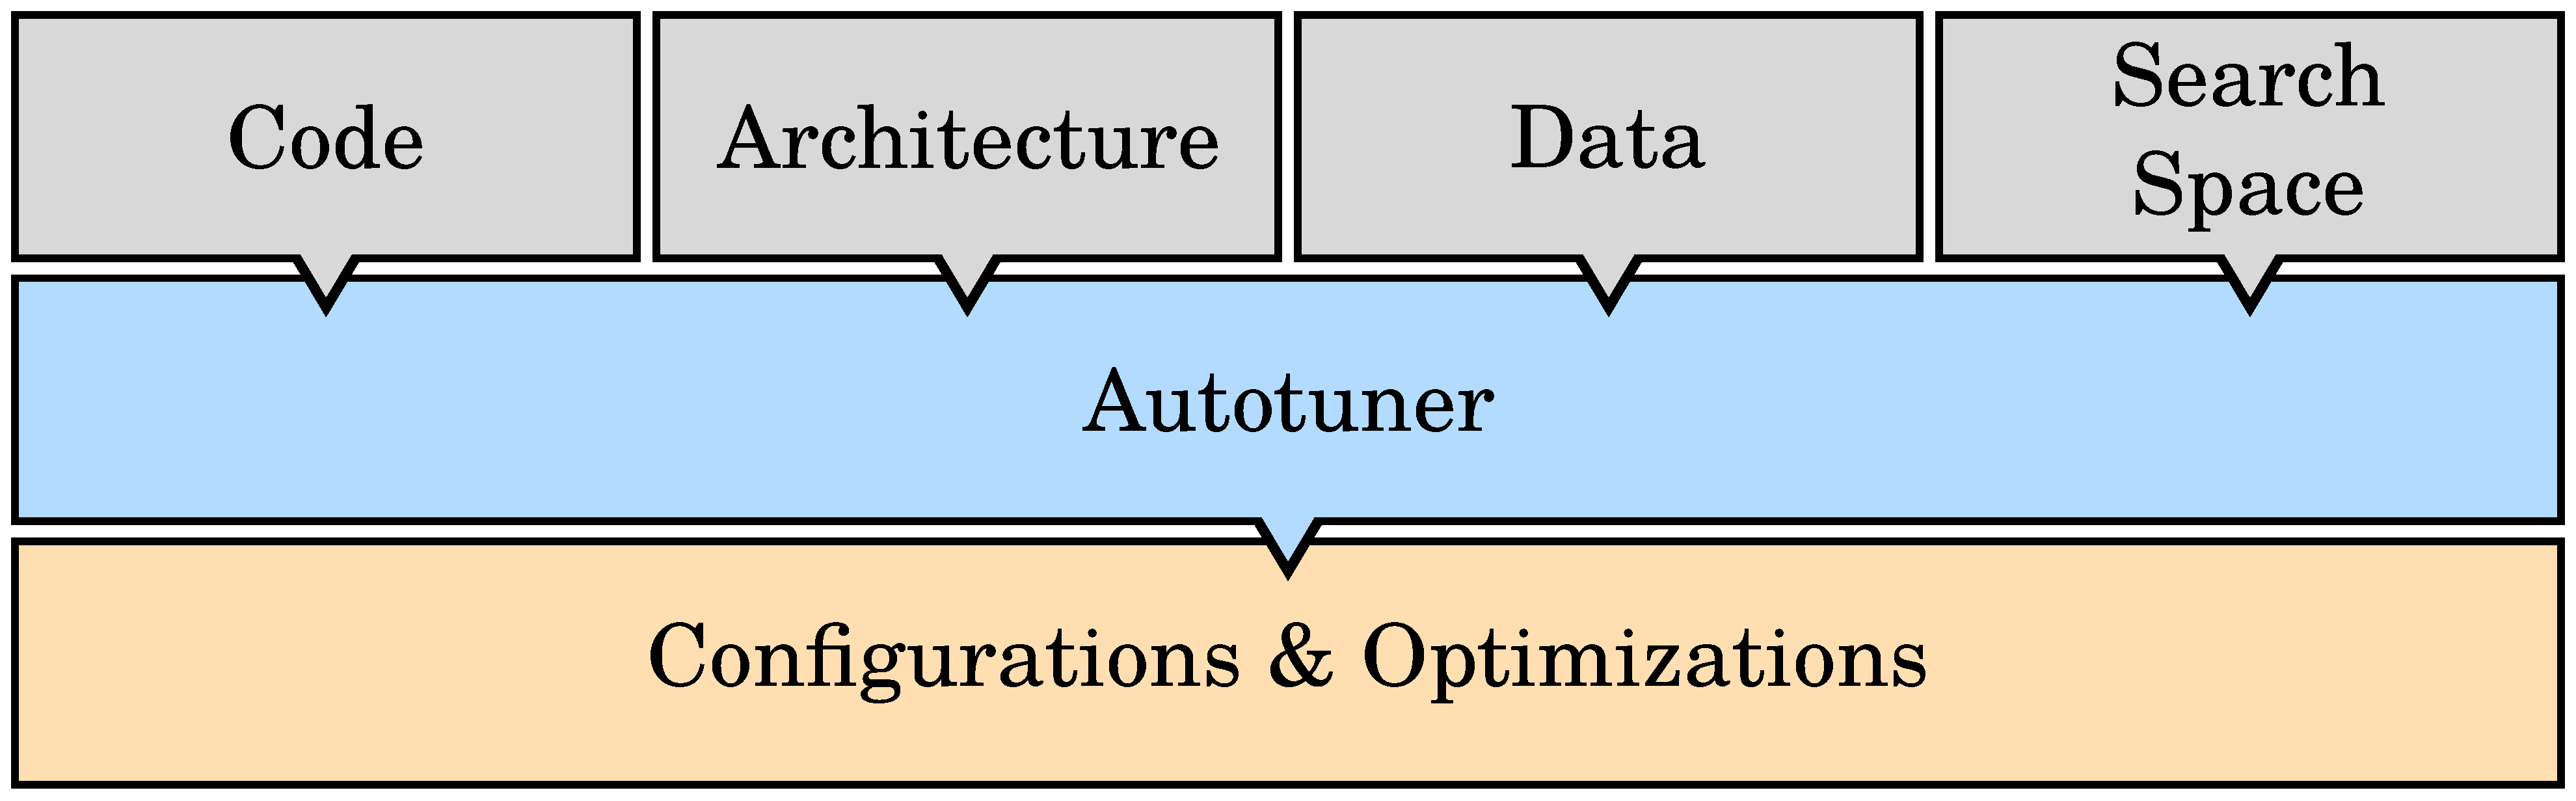
\includegraphics[width=.5\textwidth]{overview}
    \end{center}
\end{frame}

\section{Autotuning: GPU Compiler Parameters}

\begin{frame}
    \frametitle{Autotuning: GPU Compiler Parameters}
    \begin{center}
        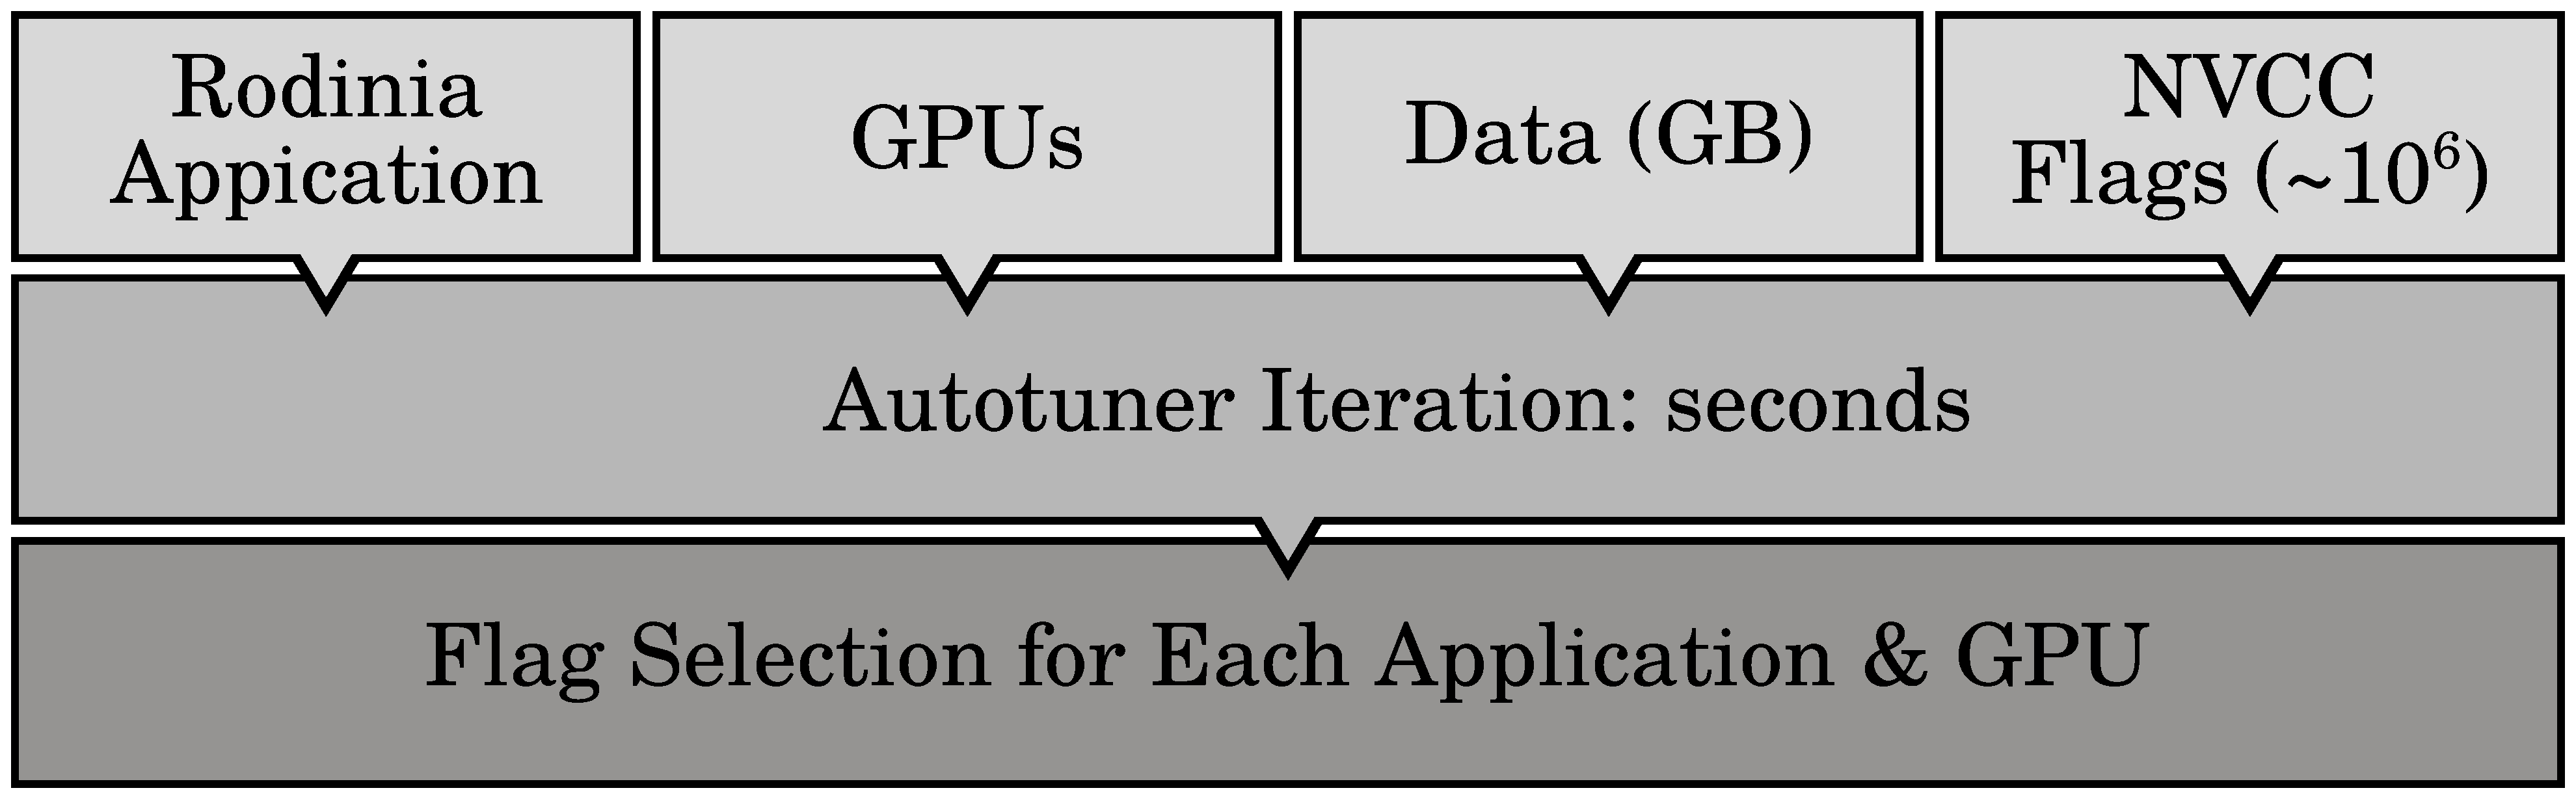
\includegraphics[width=.73\textwidth]{overview_gpus}
    \end{center}

    \begin{itemize}
        \item \alert{1h} of tuning $\approx \alert{10^3}$ \alert{iterations}
        \item From \alert{10\% to 4x speedup} vs. \texttt{-O2}
        \item \alert{Published at the CCPE Journal}
    \end{itemize}
\end{frame}

\section{Autotuning: High-Level Synthesis for FPGAs}

\begin{frame}
    \frametitle{Autotuning LegUp Parameters for CHStone}
    \begin{center}
        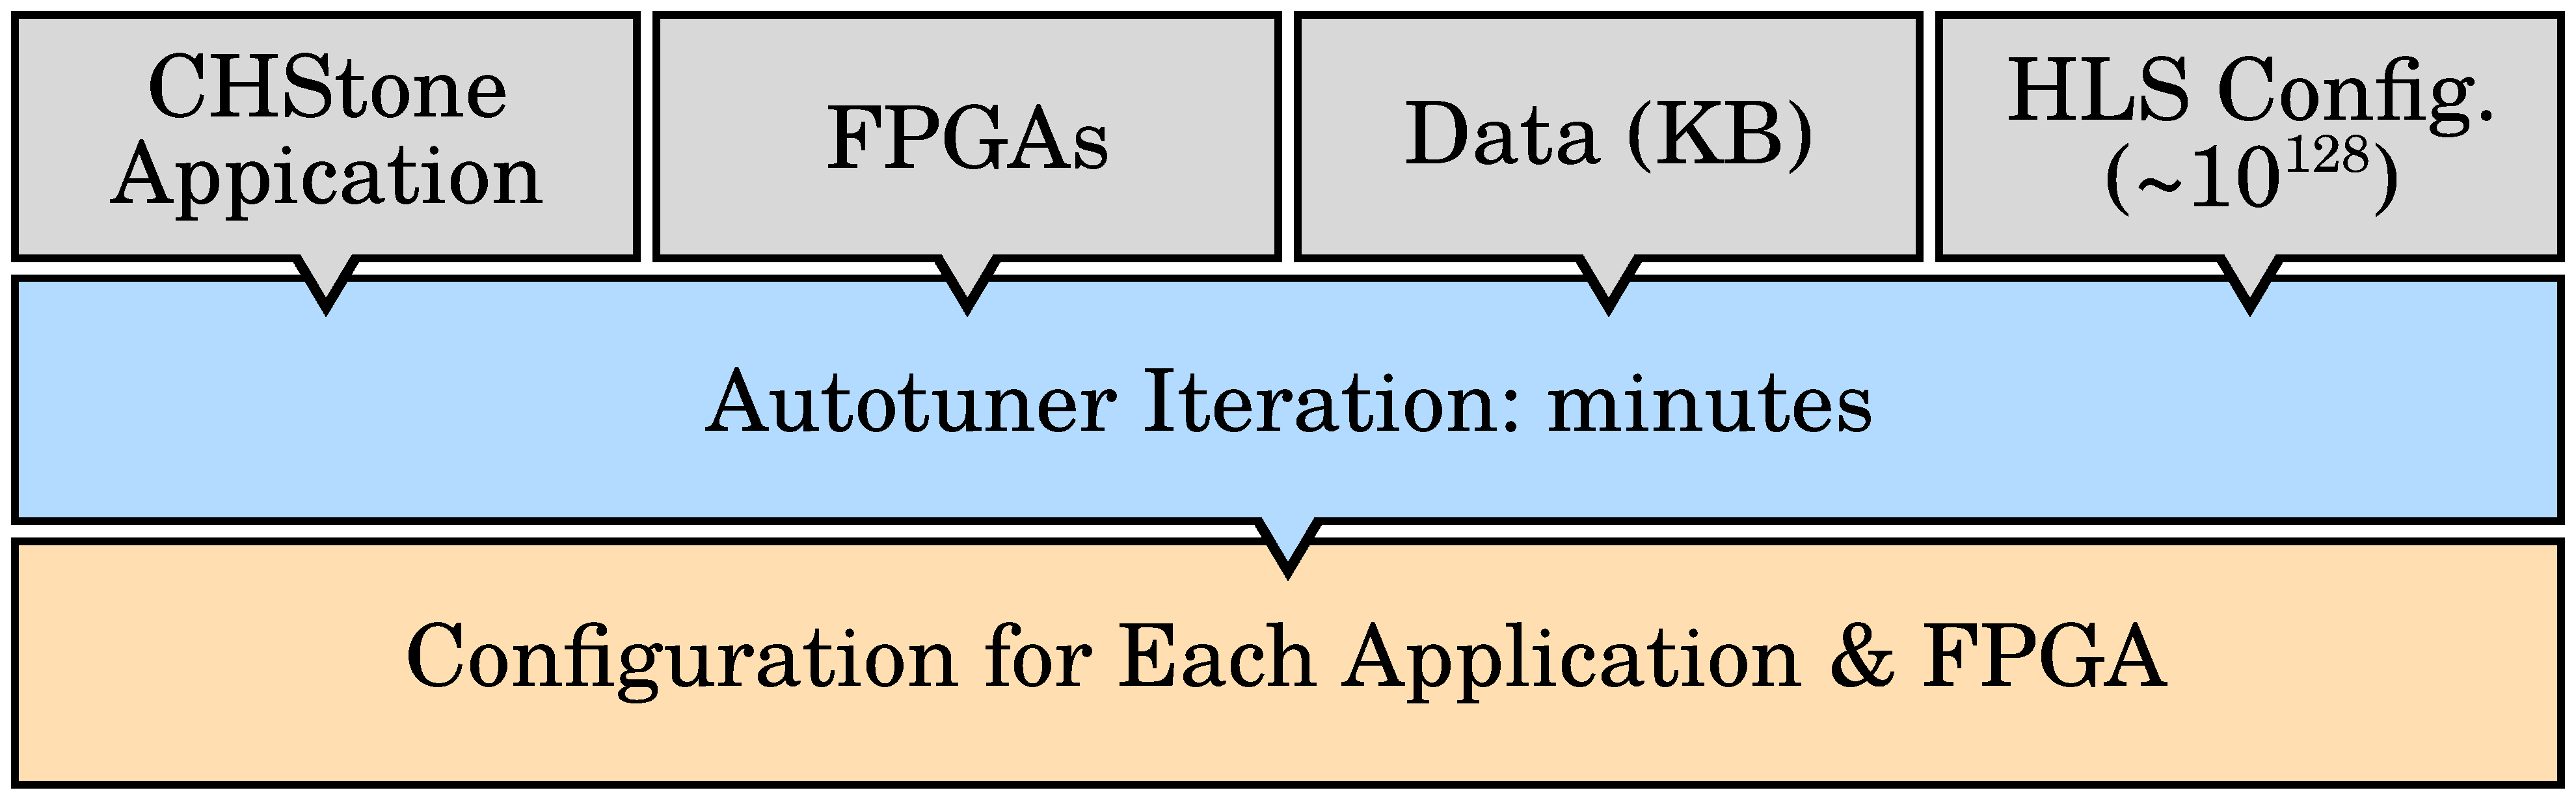
\includegraphics[width=.73\textwidth]{overview_fpgas_small}
    \end{center}

    \begin{itemize}
        \item \alert{1h} of tuning $\approx \alert{10}$ \alert{iterations}
        \item From \alert{10\% to 2x speedup}
        \item Work in progress
    \end{itemize}
\end{frame}

\section{Next Steps: Expensive-to-Evaluate Functions}

\begin{frame}
    \frametitle{Next Steps: Expensive-to-Evaluate Functions}
    \begin{center}
        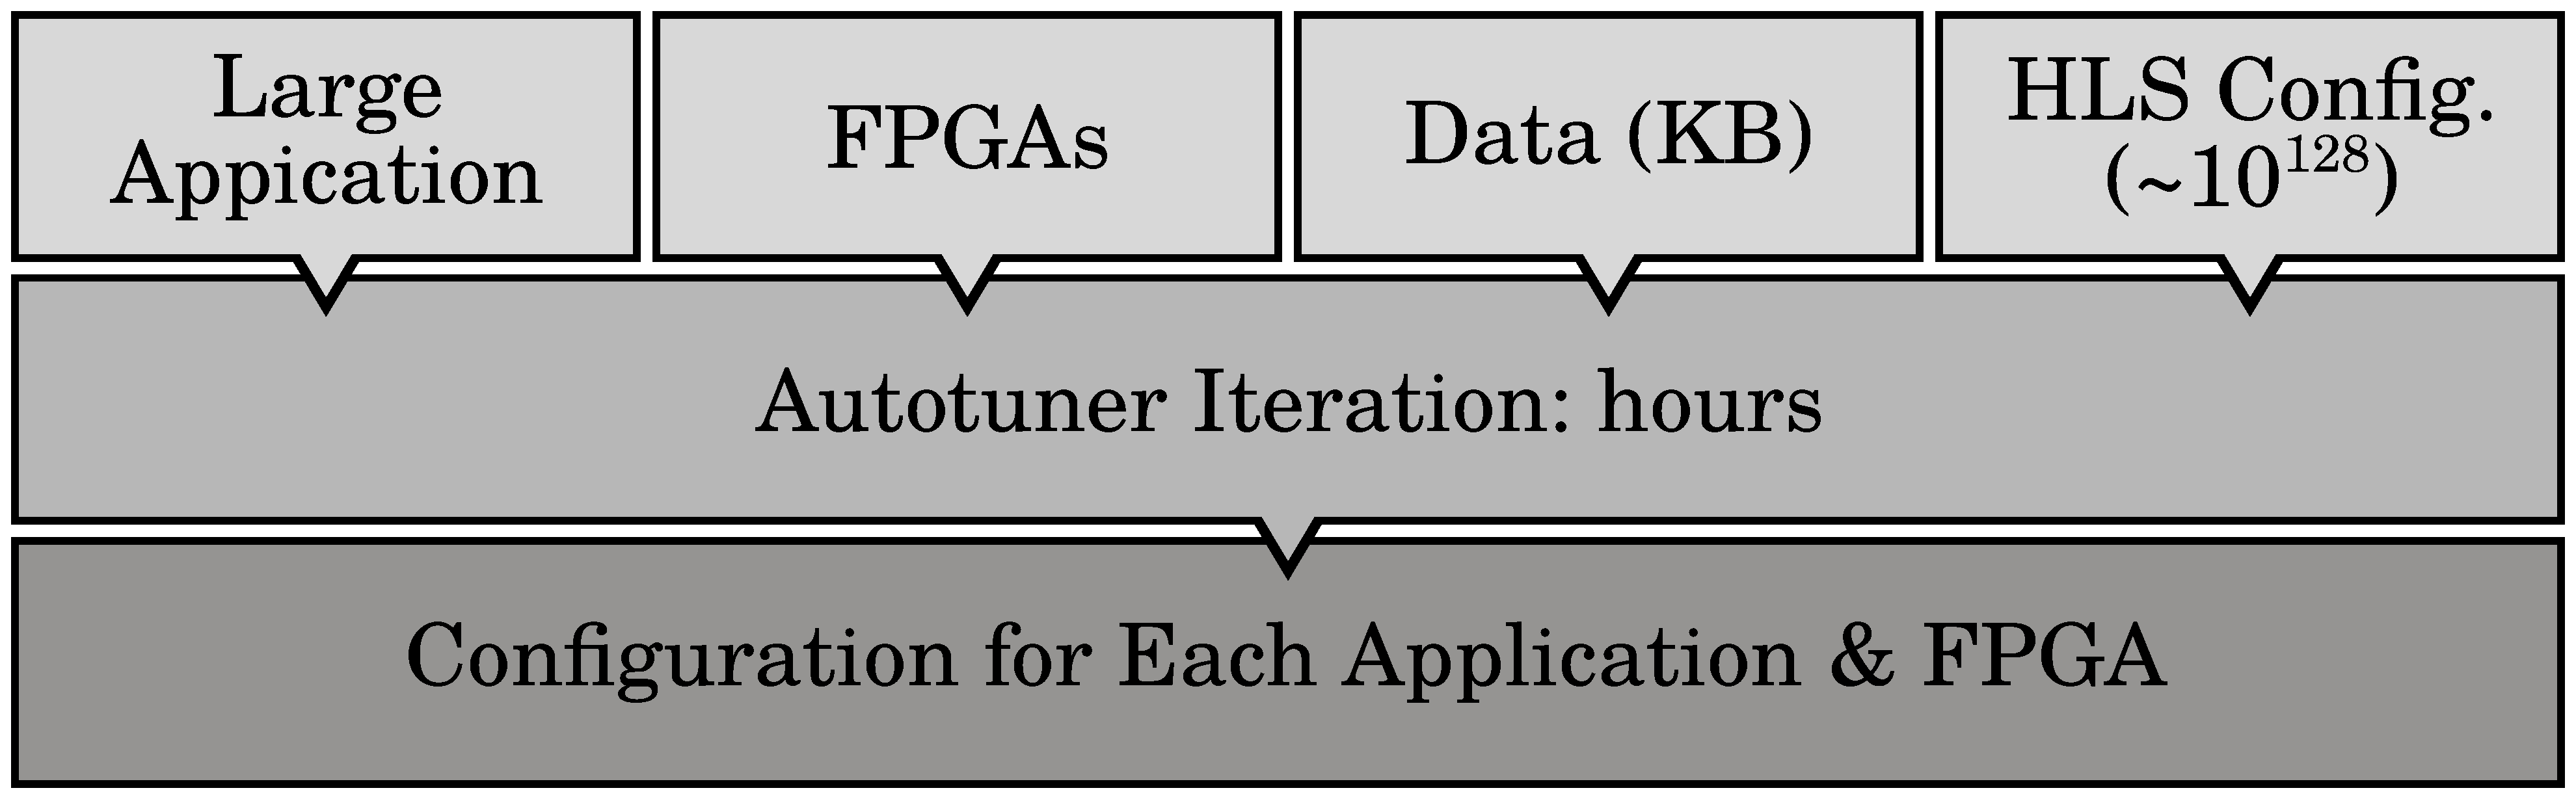
\includegraphics[width=.73\textwidth]{overview_fpgas_big}
    \end{center}

    \begin{itemize}
        \item \alert{1h} of tuning $\approx \alert{1}$ \alert{iteration}
        \item Iterations now \alert{take too long}
        \item Future work
    \end{itemize}
\end{frame}

\begin{frame}
    \frametitle{Next Steps: Parallel and Distributed Autotuning}
    \begin{center}
        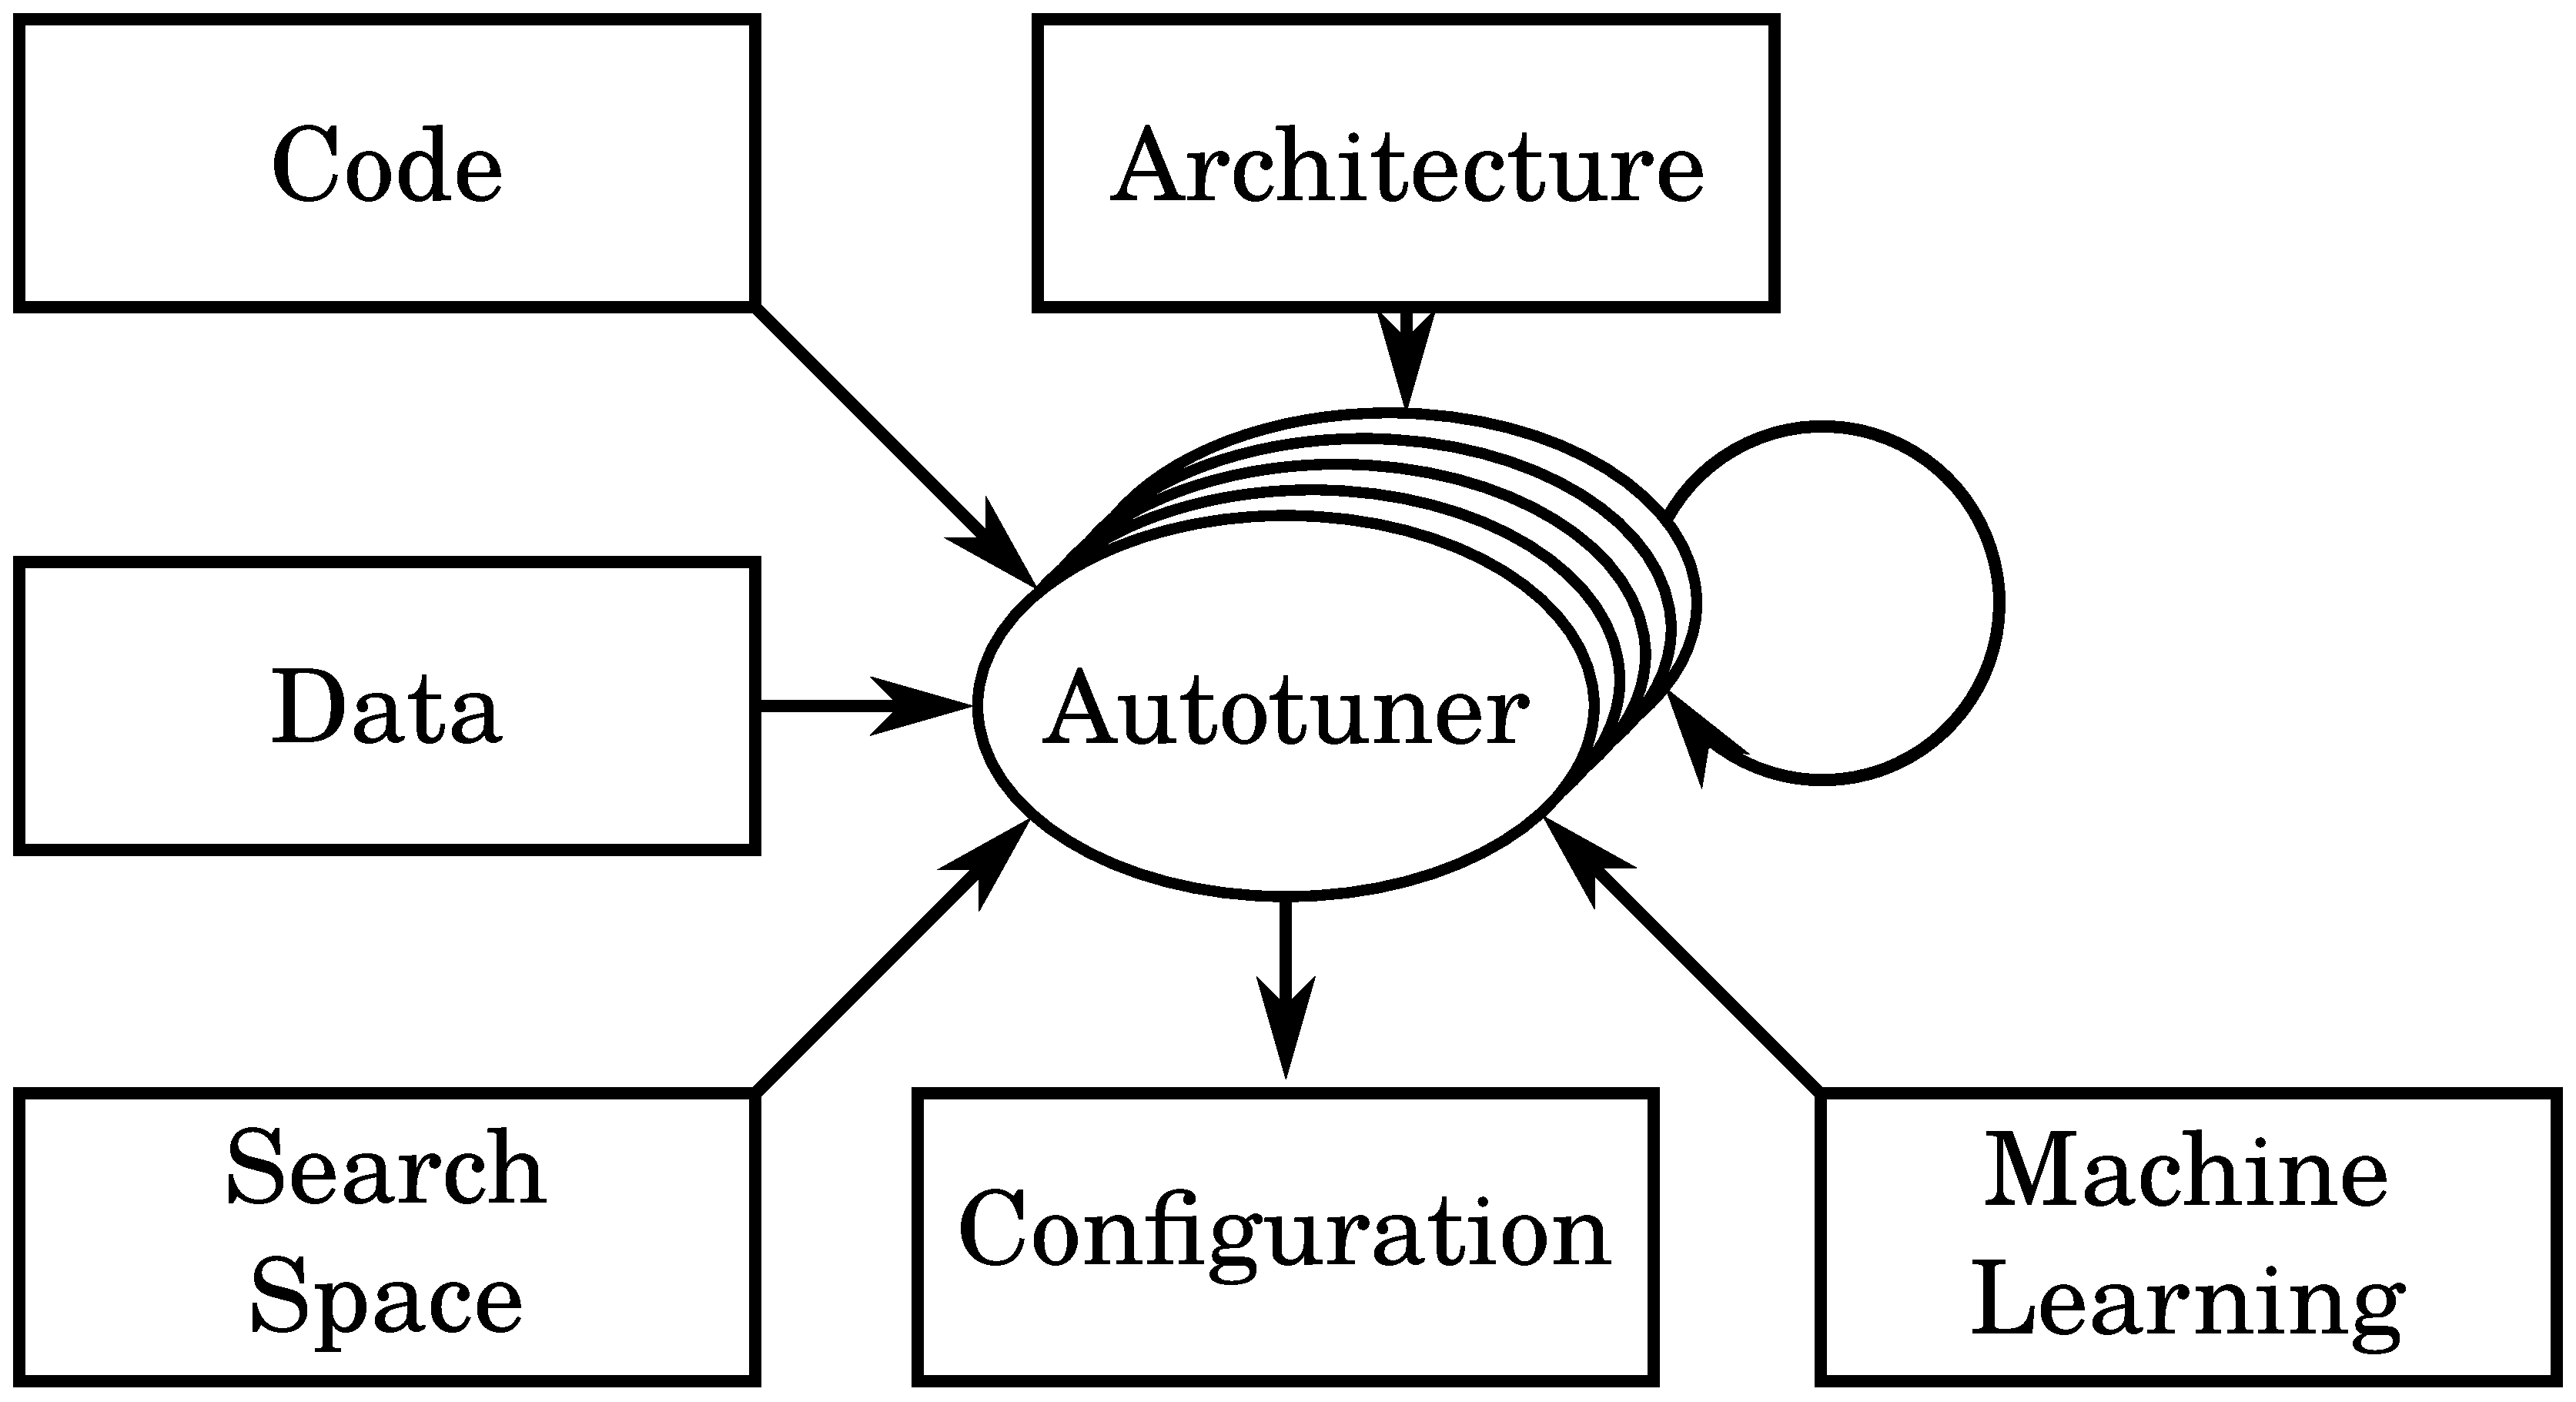
\includegraphics[width=.6\textwidth]{overview_complete}
    \end{center}
\end{frame}

\begin{frame}
    \frametitle{Next Steps: Parallel and Distributed Autotuning}
    \begin{center}
        \includegraphics[width=.3\textwidth]{ss_logo}
    \end{center}

    Domain-agnostic autotuning framework:
    \begin{itemize}
        \item \alert{Julia} language
        \item \alert{High Performance}, \alert{parallel and distributed computing}
        \item Using \alert{High-level abstractions}
        \item \alert{Expensive-to-evaluate} functions
        \item \url{github.com/phrb/StochasticSearch.jl}
    \end{itemize}
\end{frame}

\begin{frame}
    \frametitle{Next Steps: 2017 Roadmap}
    \alert{Qualification exam}:
    \begin{itemize}
        \item End of $1^{st}$ semester
    \end{itemize}

    \alert{Design of Experiments}:
    \begin{itemize}
        \item Beginning of $2^{nd}$ semester
        \item With Arnaud Legrand and Jean-Marc Vincent
        \item At Grenoble Université
    \end{itemize}

\end{frame}

\maketitle

\end{document}
